\def \imgpath {"./figures/tracks"}

This Chapter provides an overview of the triggering and data preparation procedures at the ALICE experiment. The aim is to give the reader an understanding of the process of obtaining final objects representing the particles produced in hadronic inelastic collisions at the interaction point of the LHC, utilizing the experimental apparatus that was described in the previous chapter.

\section{Events and triggers}

The ALICE experiment uses a trigger system \cite{krivdaALICETriggerSystem2012, alicecollaborationPerformanceALICEExperiment2014} to accommodate the different detector read-out times, limited data storage, and to select interesting physics events from collisions with rates of roughly $8$~kHz for Pb-Pb collisions and up to $300$~kHz for pp collisions. The Central Trigger Processor (CTP) collects input data from the trigger detectors and makes a decision about whether to take or reject the event, with the trigger decision split into three levels: L0, L1, and L2. 

The L0 trigger level makes its decision based on the fastest detectors (e.g.\ the SPD and V$0$) and sends the decision back to detectors in $\sim 1.2$~$\mathrm{\mu s}$. The L1 trigger decision is based on all remaining fast detector inputs (also including e.g.\ the Zero Degree Calorimeters located $113$~m far from the IP) and arrives back into detectors in $6.5$~$\mathrm{\mu s}$. The final L2 trigger level waits for all the detector readouts, including the slowest TPC detector, happening in about $105$~$\mathrm{\mu s}$ time. Several trigger classes can be collected simultaneously during the data taking. Once an event passes the trigger decisions of the CTP, it is sent to the Data Acquisition System (DAQ) for more detailed processing and compression of the final data.

In ALICE measurements, the following names are commonly used for some of the triggered events:
\begin{itemize}
\item \spverb|kINT7| :  the usual minimum bias (MB) class in pp collisions, based on a coincidence of the \VOA and \VOC detectors,
\item \spverb|kINT1| : also a MB class, requiring at least two signals among \VOA, \VOC, and the SPD,
\item $|$\spverb|INEL>0|$|$ : requires a MB class and at least one SPD ``tracklet" within $|\eta|<1$, which is reconstructed in the two SPD layers.
\end{itemize} 

\section{Event and track reconstruction}

Reconstruction of the event information in the central barrel follows a procedure discussed in Ref.~\cite{} and summarised in Fig.~\ref{fig:tracks:flow}. It begins with clusterisation, where the detector data is transformed into clusters, or \textit{reconstruction points}, that include the spatial information, signal amplitude, signal time, and associated errors. The clusterisation is carried out locally for each detector, for instance, for the TPC, a cluster corresponds to a crossed row in the ROCs.  The next steps are discussed in this section.


--
Next, preliminary primary vertex (PV) is determined by utilising clusters in the first two ITS layers (SPD). The Kalman filter technique is employed to perform track finding and fitting in TPC and ITS. The discovered tracks are then matched to other detectors in the central barrel and fitted. The reconstructed tracks are used to determine the final interaction vertex. The central-barrel tracking procedure concludes with a search for photon conversions, strange hadron decays (K0
S/Λ, Ξ±, and Ω±), and V0 particles. The steps are discussed in greater detail in this section.

\begin{figure}%[!h]
\adjincludegraphics[trim={0 {.68\height} 0 {.07\height}},clip,width=.99\textwidth]{\imgpath/flow.pdf}
\caption{Work flow diagram of the event information reconstruction in the central barrel. \cite{LHCReportMake2023}}
\label{fig:tracks:flow}
\end{figure}

\subsection{First primary vertex determination}

A preliminary primary vertex (PV) is determined using tracklets formed in the two SPD layers of the ITS. A three-dimensional reconstruction is performed in pp and pA collisions, iteratively, so that events with in-bunch pile-up can be treated. With each iteration, clusters with tracklets already pointing to a vertex are removed. By construction, the first found vertex has the highest number of corresponding tracklets and is defined as primary. The If this method fails, the PV is determined only in the $z$-dimension. This is also the default in AA collisions. These methods are visualised in Fig.~\ref{fig:tracks:pvfirst}.

\begin{figure}%[!h]
\subfloat[][]{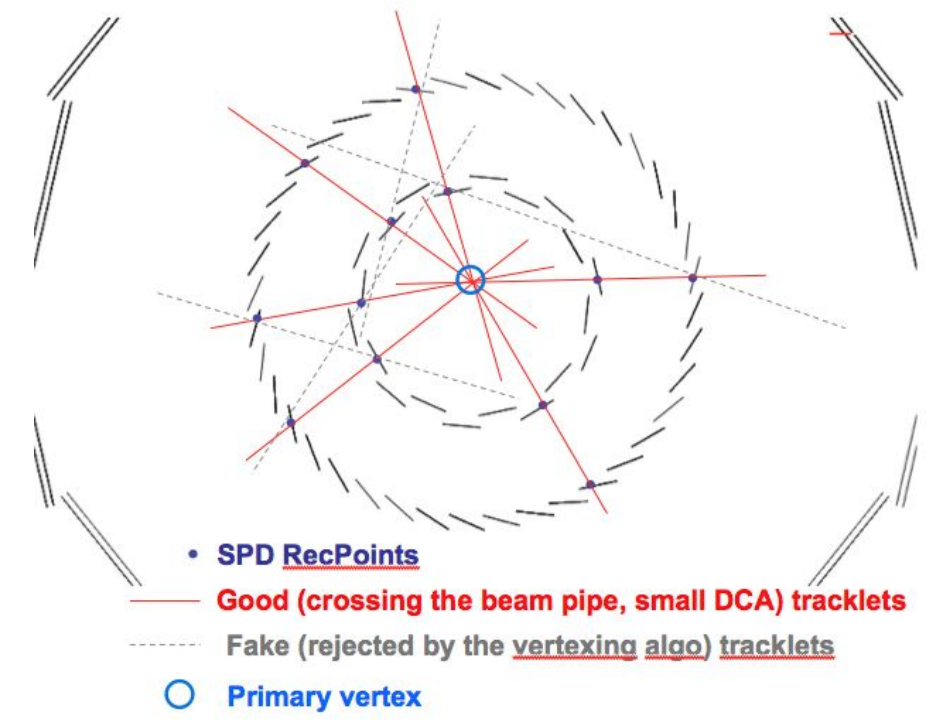
\includegraphics[width=.35\textwidth]{\imgpath/pv1.png}}\hspace{3em}
\subfloat[][]{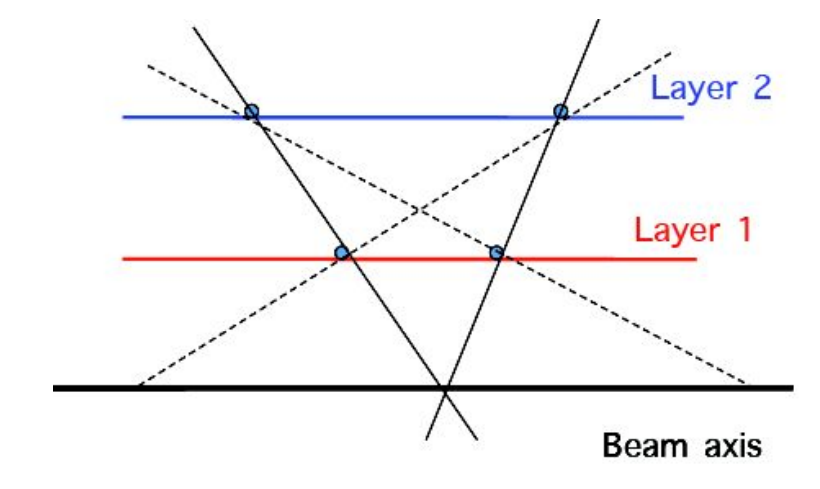
\includegraphics[width=.35\textwidth]{\imgpath/pv2.png}}
\caption{\textbf{(a)} Preliminary three-dimensional reconstruction of the primary vertices, also depicting tracklets rejected by the algorithm. \textbf{(b)} Preliminary one-dimensional reconstruction of the PVs. \cite{alicedatapreparationgroupALICEDataFlow2018}}
\label{fig:tracks:pvfirst}
\end{figure}

\subsection{Tracking}

Track finding (recognition) and track fitting (reconstruction) is carried out simultaneously using the Kalman filter technique in three steps: inwards, outwards, inwards \cite{arslandokTrackReconstructionHighDensity2022}. The entire process is illustrated in Fig.~\ref{fig:tracks:tracking}. 

First, for \textit{primary} tracks, i.e.\ tracks hypothesised to originate from the PV, seeds are found from the preliminary SPD PV and pairs of TPC clusters at the highest radii, where track densities are the lowest. For \textit{secondary} tracks, coming for instance from weak decays with displaced secondary vertices, three TPC clusters are used instead of considering the PV. The track seeds are then projected inwards, adding clusters fulfilling given proximity cuts, and updating the track parameters at each step, until the inner TPC radius is reached. Preliminary $\mathrm{d}E/\mathrm{d}x$ is also stored. Moreover, tracks sharing multiple clusters (approx.\ more than $25\%$) are discarded in favour of their higher-quality doubles. 

The TPC tracks are then extrapolated to the ITS, where they continue to get updated. This tracking efficiency in the TPC, displayed in Fig.~\ref{fig:alice:pres}, drops significantly below $\approx \mevc{200}$, where energy loss and multiple scatterings start playing a role. For this reason, the ITS also runs a standalone Kalman filter algorithm, using clusters that are not associated with the TPC track. There, similarly to the TPC, candidates are considered both with and without a PV constraint.

In the second step, tracks are extrapolated to the point of closest approach (PCA) with respect to the PV and back-propagated to the TPC outer radius, using the previously added clusters. Now, track lengths are also considered and an expected time-of-flight (TOF) information is calculated based on the stored $\mathrm{d}E/\mathrm{d}x$. The tracks are then extrapolated to the Transition Radiation Detector (TRD), TOF, and possibly other detectors with clusters, where they can be matched with them. The ITS standalone tracks are propagated only to the ITS outer radius.

Finally, the tracks udpated with the TRD and TOF (and possible other) information are re-fitted in each detector inwards again, starting at the TPC outer radii and propagating to the PV PCA. As a result of using the Kalmar filter, the track parameters are then finalised and given unambiguously, at the point of the primary vertex. More than $90\%$ of the reconstructed tracks are primary tracks. This ratio can be significally enhanced by imposing transverse and longitudinal cuts on the distance of closest approach (DCA) to the PV.

\begin{figure}[!h]
\subfloat[][]{\adjustbox{valign=m}{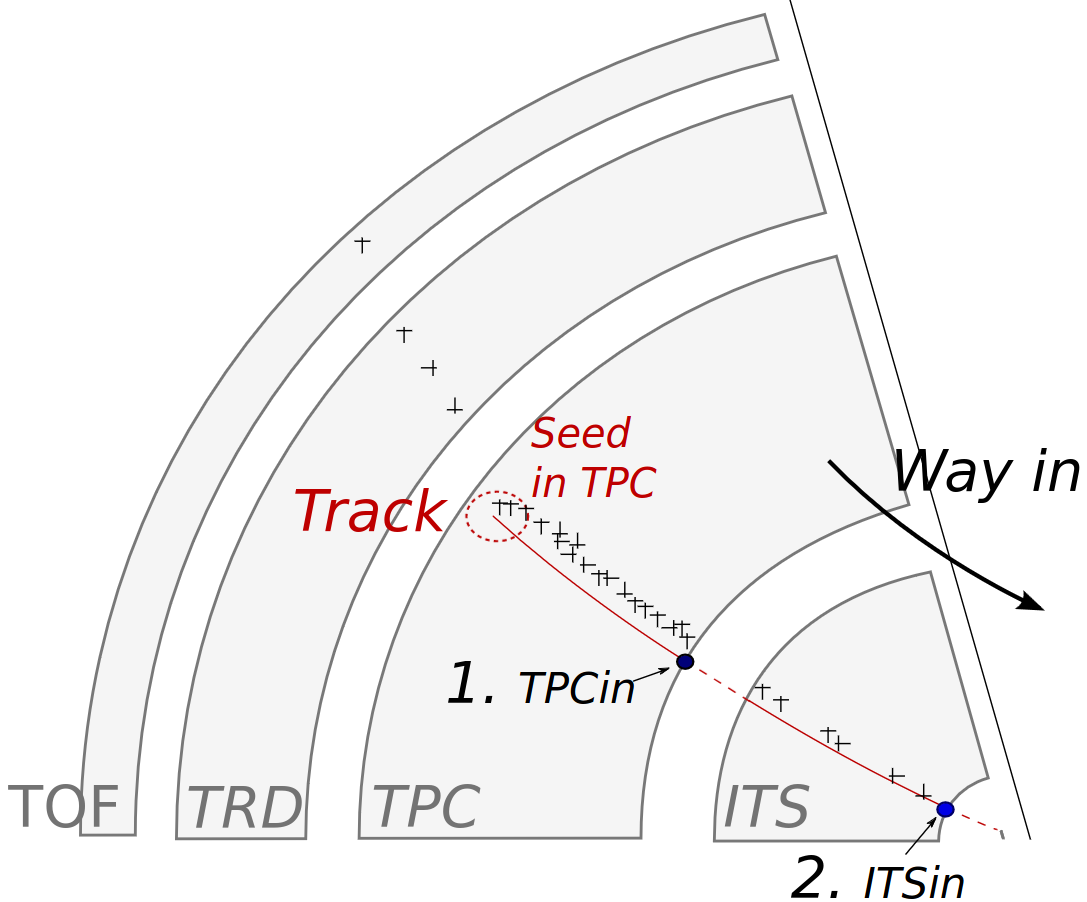
\includegraphics[width=.38\textwidth]{\imgpath/first.png}}}\hspace{1em}
\subfloat[][]{\adjustbox{valign=m}{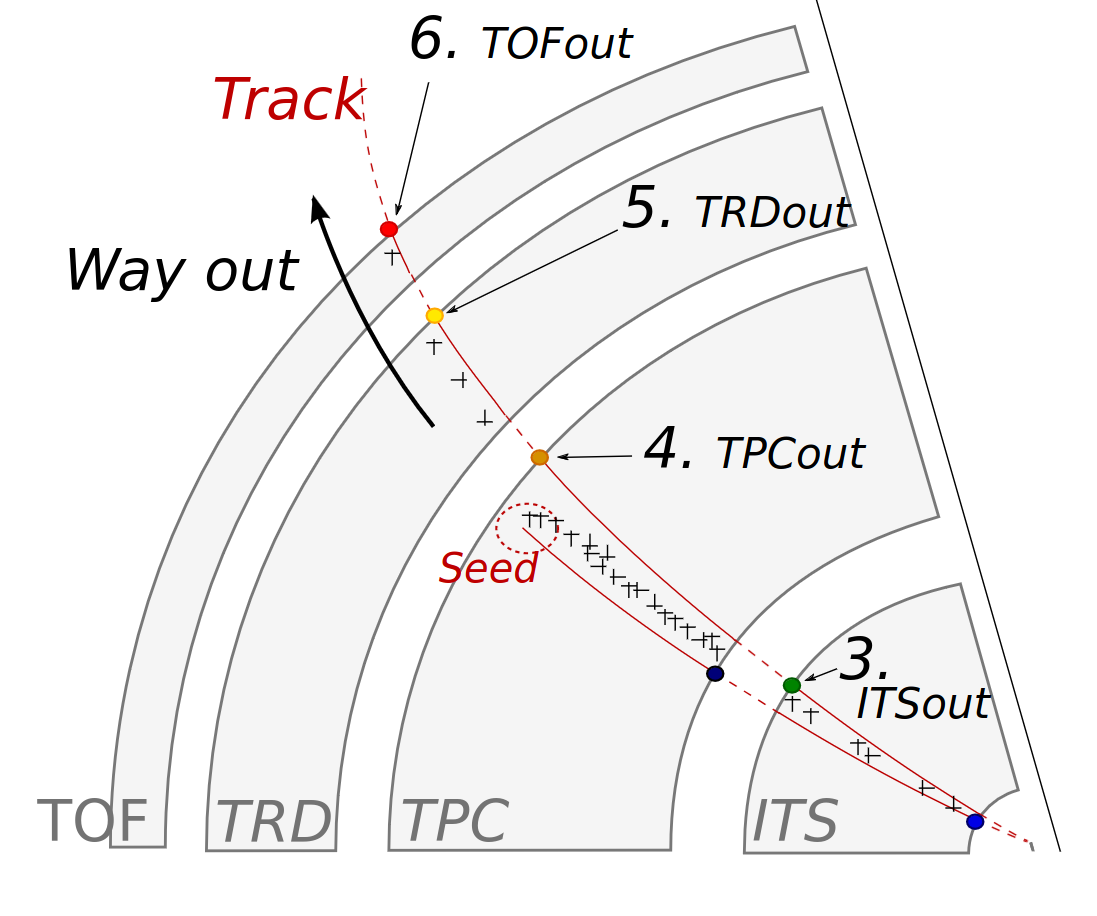
\includegraphics[width=.38\textwidth]{\imgpath/second.png}}}\\
\subfloat[][]{\adjustbox{valign=m}{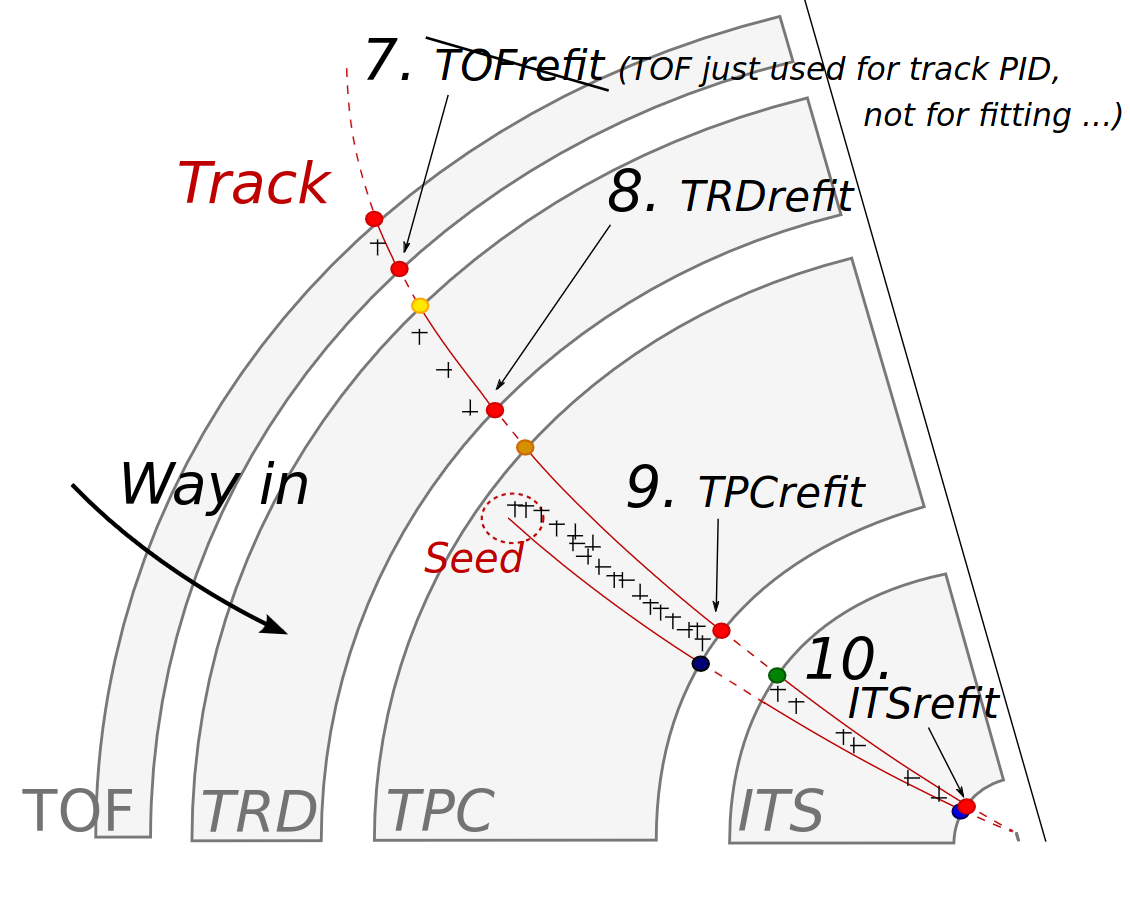
\includegraphics[width=.38\textwidth]{\imgpath/third.png}}}
\caption{Diagrams illustrating the inward-outward-inward approach in central barrel tracking. \textbf{(a)} First: track seeding and propagation to ITS and PV. \textbf{(b)} Second: back-propagation through ITS and TPC and extrapolation to TRD and TOF. \textbf{(c)} Third: final re-fit. \cite{maireProductionBaryonsMultietranges2011}}
\label{fig:tracks:tracking}
\end{figure}

The ITS- and TPC-combined tracks enjoy the highest momentum resolution, which is plotted as a function of the track \pt in Fig.~\ref{fig:tracks:pres}. It corresponds to values of about $1\%$ at \gevc{1} and then continues increasing as higher-\pt tracks are less curved, thus less constrained, and more likely to have a larger part in the detector's inactive regions. The disadvantage of the ITS-TPC tracks is their azimuthal non-uniformity due to gaps in the ITS acceptance, particularly the SPD.

\subsubsection*{Final PV determination}

Subsequently, the ITS-TPC \textit{global} tracks are used to determine the PV with a higher precision than when using the SPD tracklets alone. Tracks are also weighted to minimise the effect of outliers and the nominal beam position can also be used as a space point. In high pile-up runs, an iterative vertex process is performed. Standard deviation of the vertex position in the transverse region ranges from $\sim 1$~mm in events with one track to $\sim 0.1$~mm in events with five tracks and more.

\begin{figure}[!h]
\subfloat[][]{\adjustbox{valign=m}{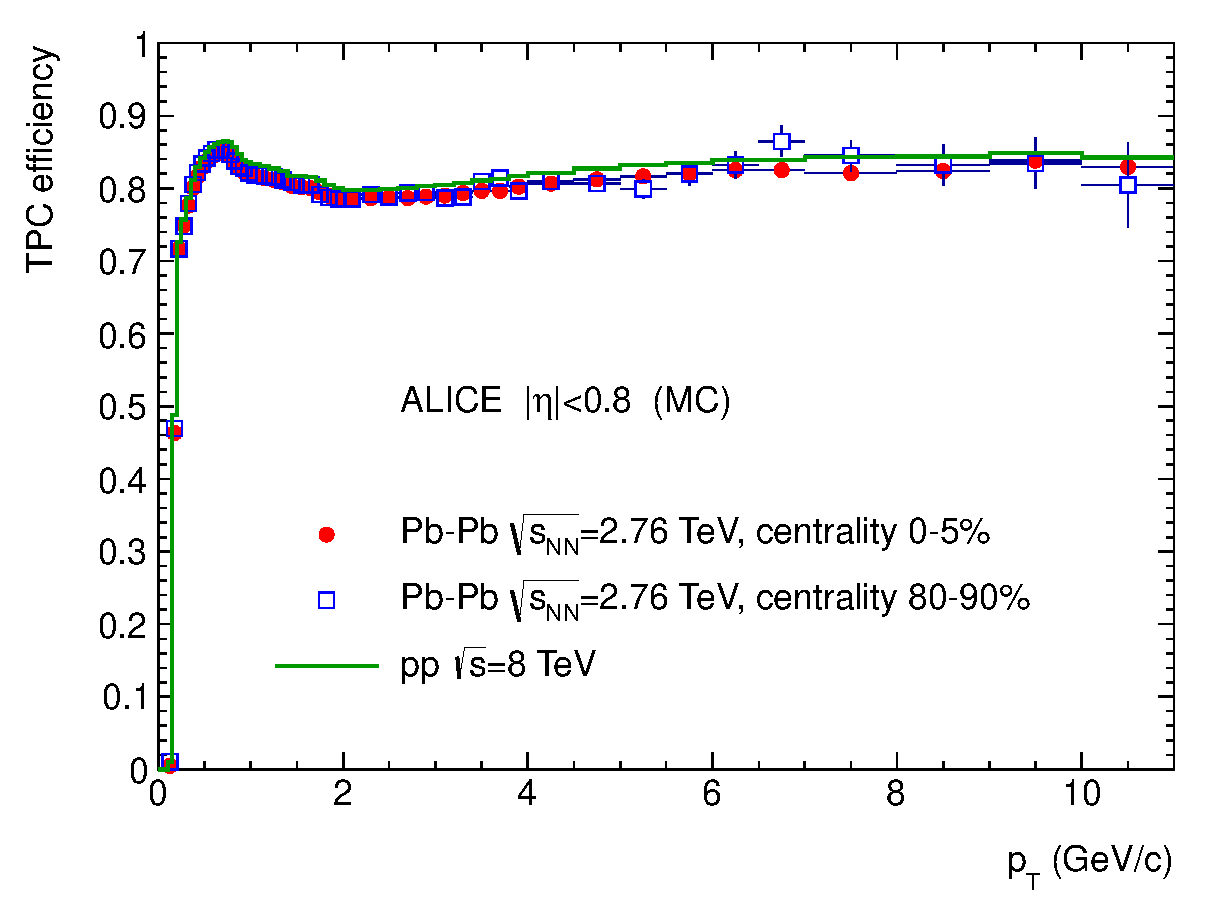
\includegraphics[width=.46\textwidth]{\imgpath/tpceff.eps}}}\hspace{1em}
\subfloat[][]{\adjustbox{valign=m}{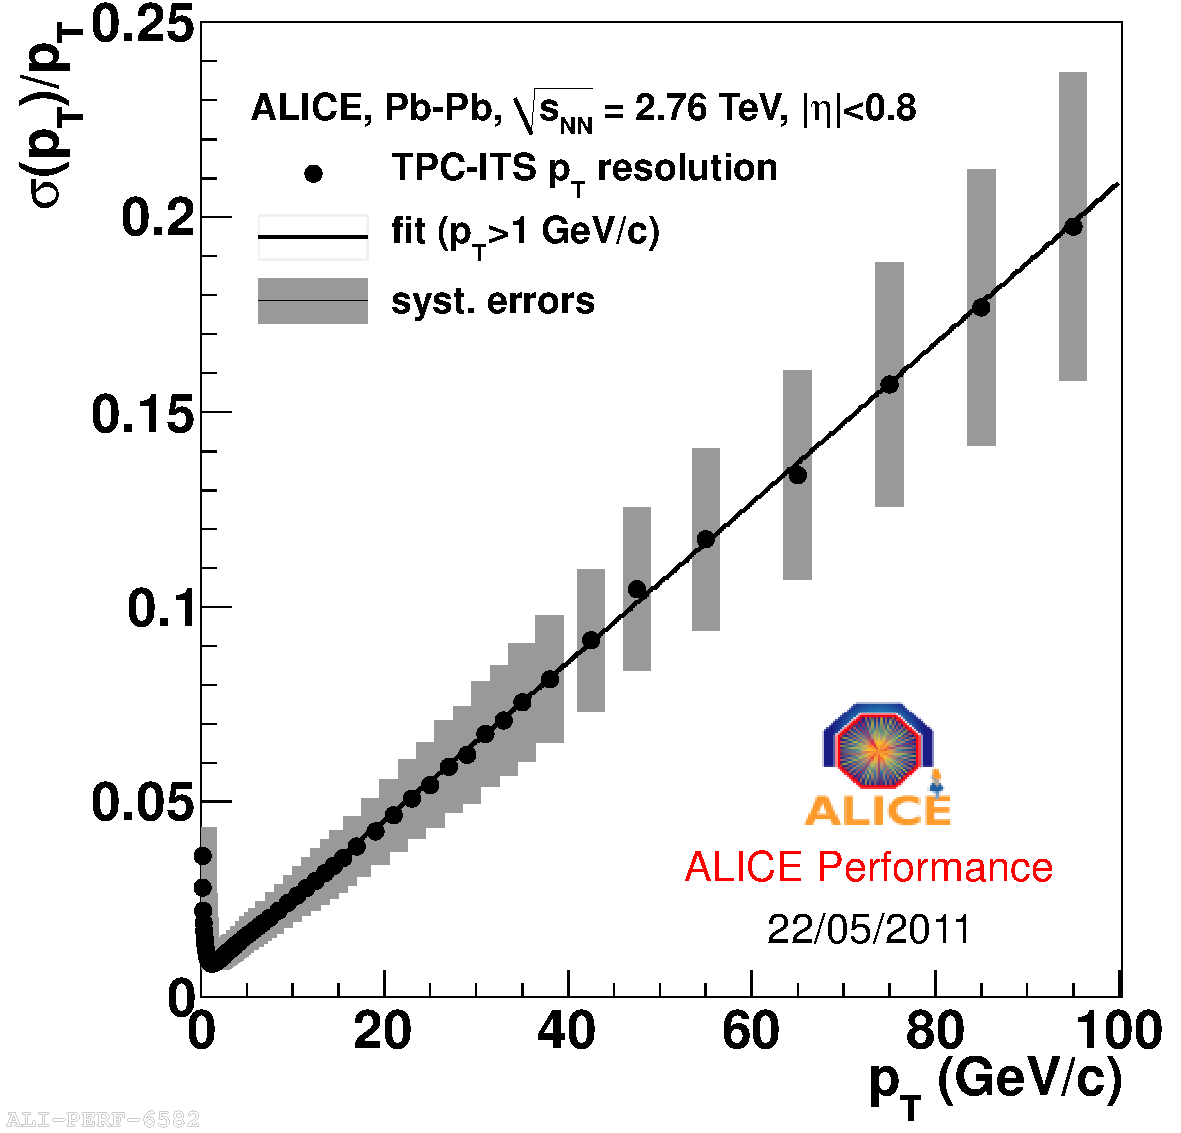
\includegraphics[width=.40\textwidth]{\imgpath/reso.pdf}}}\\
\caption{\textbf{(a)} Efficiency of track finding in the TPC for primary particles in pp collisions (green) and Pb-Pb collisions at different centralities (blue and red), determined from simulations. \cite{alicecollaborationPerformanceALICEExperiment2014} \textbf{(b)} Transverse momentum resolution of the combined ITS-TPC tracking in Pb-Pb collisions. \cite{continPerformancePresentALICE2012}}
\label{fig:tracks:pres}
\end{figure}

\subsection{Finding secondary vertices}

After the track and primary vertex reconstruction, an algorithm is ran to find secondary vertices corresponding to photon pair conversions, the so-called \VOs (weak decays of e.g.\ the \KOs and \LA) and the so-called \textit{cascades} (\XI and $\Omega$),  based on the topology shown in Fig.~\ref{fig:tracks:topo}. First, pairs of unlike-signed tracks with a given DCA with respect to the PV are formed (more than $0.5$~mm in pp or $1.0$~mm in Pb-Pb). Furthermore, loose cuts on the topology of the decay (discussed in more detail in Chapter~\ref{chap:analysis}) are imposed. Specifically, 
\begin{enumerate}
\item the PCA of the two tracks with respect to each other needs to be closer to the PV than the inner-most cluster of either of them, which corresponds to the fact that the daughters are produced in the vertex,
\item the DCA of the two tracks needs to be smaller than $1.5$~cm,
\item if the two-track momentum exceeds $\pt>\gevc{1.5}$, cosine of the \textit{pointing angle} (CPA) between the formed momentum vector and the straight line connecting the two-track PCA and the PV needs to be larger than $0.9$.
\end{enumerate}

The \VOs search can occur ``online" during the tracking, using a full information of the clusters, or ``offline", at a later stage, where it is based on the reconstructed tracks and can be re-configured. Subsequently, a search for cascades is performed: the found secondary vertices are matched with other secondary \textit{bachelor} tracks if
\begin{enumerate}
\item the invariant mass of the found pair is consistent with that of a \LA, assuming a p and $\pi$ mass hypothesis for the two tracks,
\item the bachelor DCA to the PV exceeds $0.2$~cm.
\end{enumerate}

%Improved finder

\begin{figure}%
\includegraphics[width=.590\textwidth]{\imgpath/v0.eps}\\
\caption{Diagram showing topology of a \VO decay (in this case \KOs) and a cascade decay (in this case \XI) in the central barrel. Here, the decays occured within the ITS volume, but this is not a requirement for the reconstruction. The radii are not to scale. \cite{alicecollaborationPerformanceALICEExperiment2014}}
\label{fig:tracks:topo}
\end{figure}

\section{Centrality and multiplicity measurements and their caveats}

In Pb-Pb collisions, the experimentally measured multiplicity can be related to the centrality using the Glauber picture, as discussed in Chapter~\ref{chap:colls}, which maps the final state to the percentage of the total hadronic cross section based on the collision geometry. This picture assumes that the multiplicity due to the different \Npart dominates over contributions from specific event sub-structures (e.g.\ a hard jet), and that the effect of fluctuations is small enough to play a role. In ALICE, this procedure is performed typically using the \VOM estimator (as it has the highest centrality resolution \cite{alicecollaborationPerformanceALICEExperiment2014}). The \VOM is a summed amplitude in the two \VOA and \VOC forward-rapidity scintillators, and the mapping procedure is discussed in detail in e.g.\ Ref.~\cite{alicecollaborationCentralityDeterminationPbPb2013}.

Apart from the \VOM, multiplicity can also be estimated at mid-rapidity, using the SPD, which allows for taking into account particles with even very low momenta. This can be defined as either
\begin{itemize}
\item the number of clusters in the first layer of the SPD, also known as \spverb|CL1|,
\item or the number of formed tracklets in the SPD at $|\eta < 0.8$. This is also used in the studies done in this thesis and is referred to as \NSPD.
\end{itemize}

In pp collisions, the choice of mid-rapidity estimators comes with an important caveat when measuring particle spectra. Since event classification and tracking are performed in the same region, and fluctuations are not negligible compared to the multiplicities, an auto-correlation bias occurs. This can be seen in Fig.~\ref{fig:tracks:ktok}, which compares the integrated yields of charged kaons to neutral \KOs, scaled by a factor of two. As the multiplicity increases, the two yields become different, because requiring a large number of charged particles to classify the event as high multiplicity biases the charged kaon yields to higher values.

Furthermore, it should be noted that apart from this auto-correlation bias, spectra measured as a function of mid-rapidity and forward-rapidity multiplicity may still exhibit differences, as the choice of rapidity also plays a role when accessing and classifying the underlying dynamics of particle production in the event. This is illustrated in Fig.~\ref{fig:tracks:nmpi}, which shows a different dependence of the mean number of MPIs \meannmpi in Pythia 8 on the multiplicity selected by the two classifiers.

\begin{figure}[!h]
\subfloat[][]{\adjustbox{valign=m}{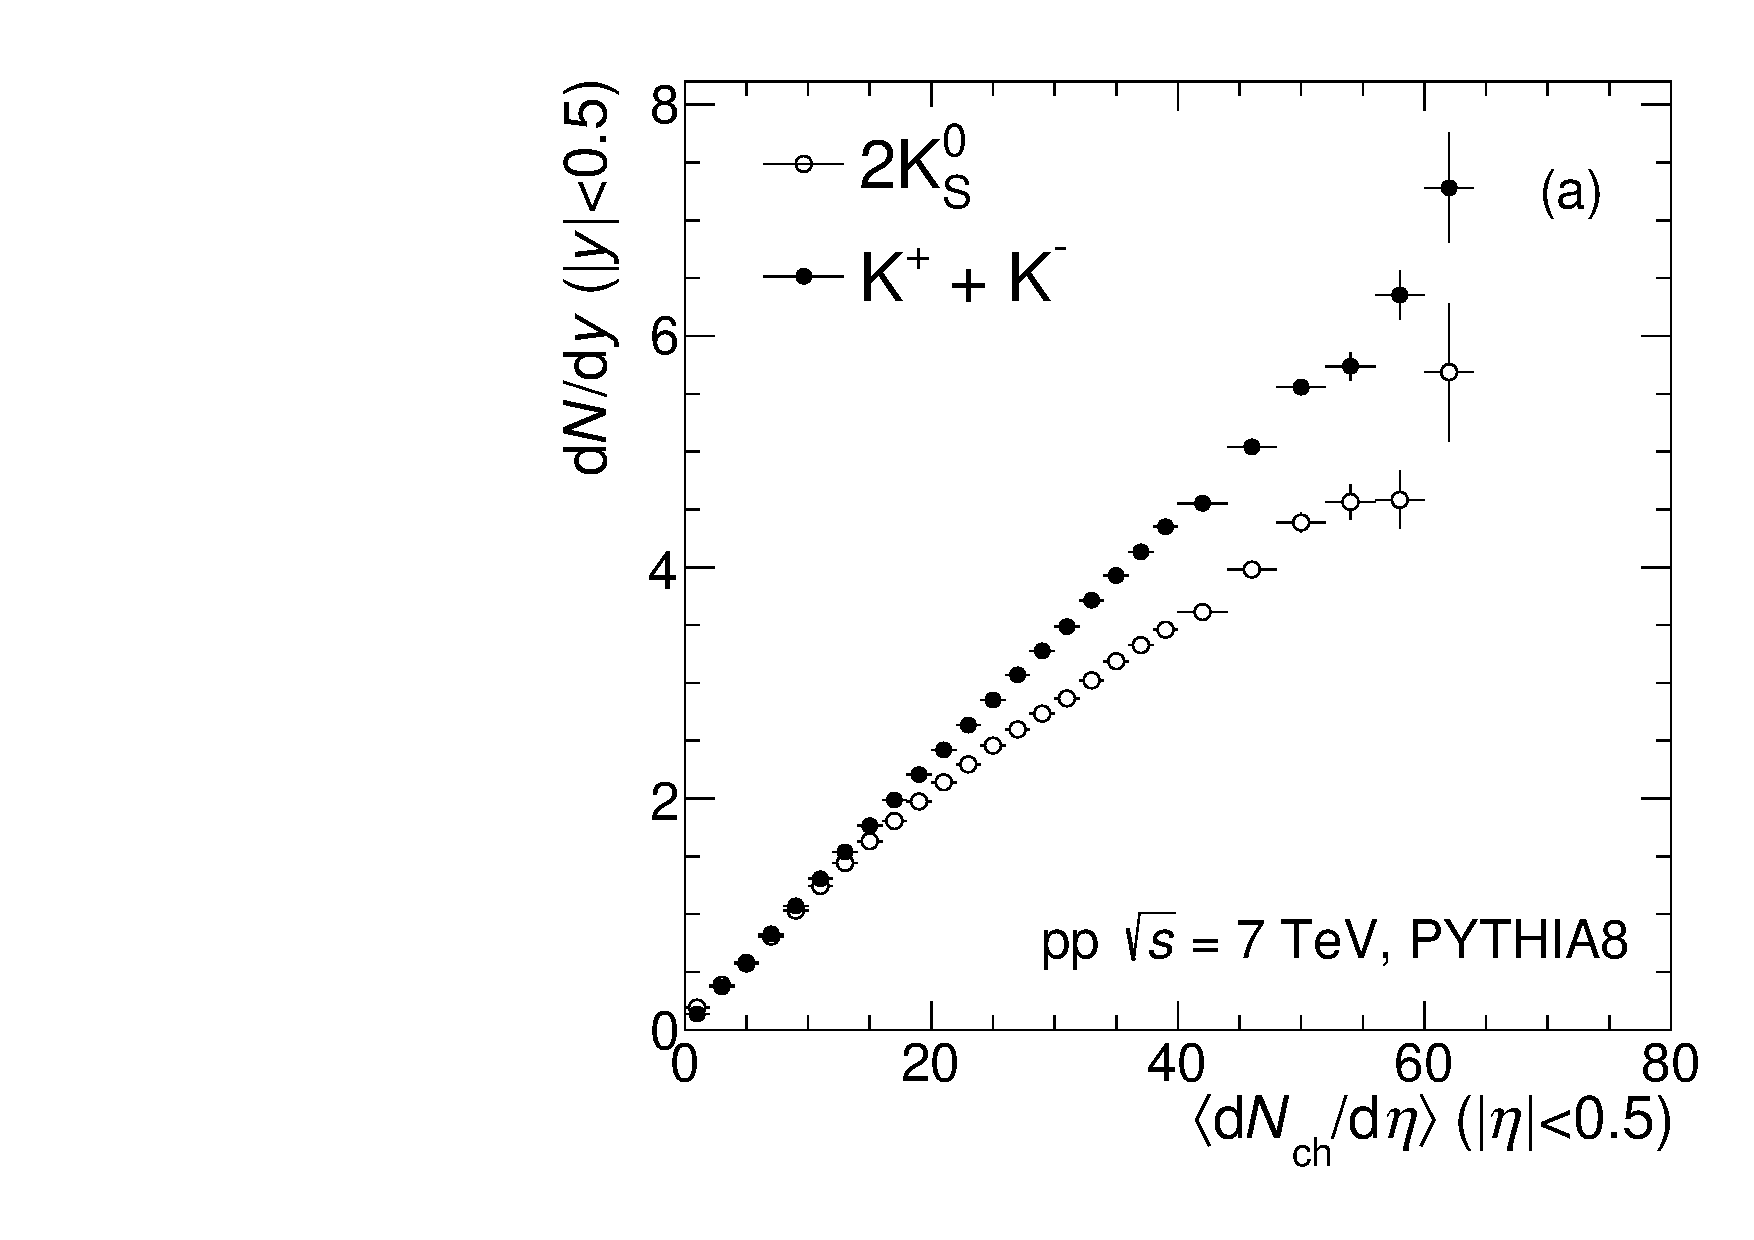
\includegraphics[width=.40\textwidth]{\imgpath/ktok_nch.pdf}}}\hspace{1em}
\subfloat[][]{\adjustbox{valign=m}{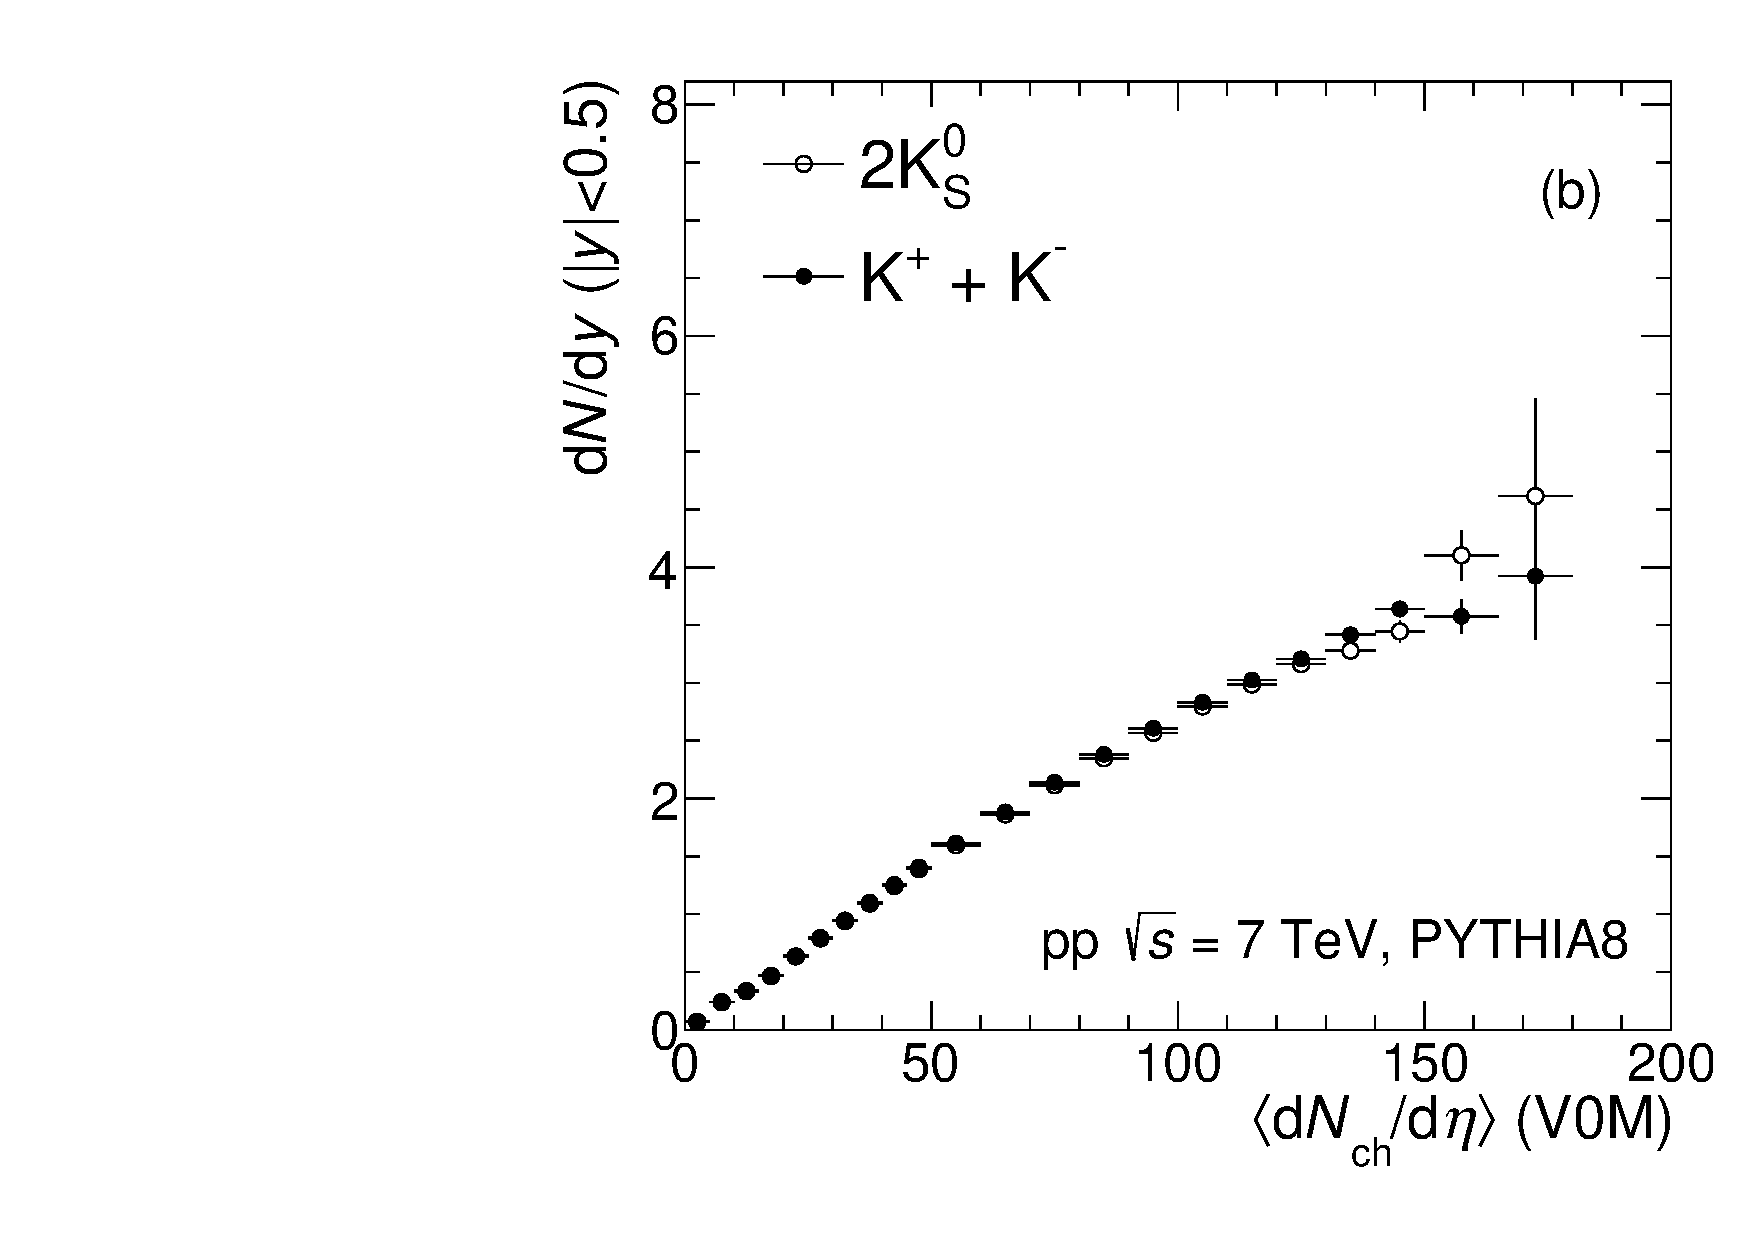
\includegraphics[width=.40\textwidth]{\imgpath/ktok_vom.pdf}}}\\
\caption{Dependence of charged and neutral kaon yields in pp collisions on the multiplicity determined \textbf{(a)} at mid-rapidity using the \NSPD estimator and \textbf{(b)} at forward rapidity using the \VOM estimator, as simulated by Pythia 8. \cite{alicecollaborationMultiplicityDependenceLightflavor2019}}
\label{fig:tracks:ktok}
\end{figure}

\begin{figure}[!h]
\subfloat[][]{\adjustbox{valign=m}{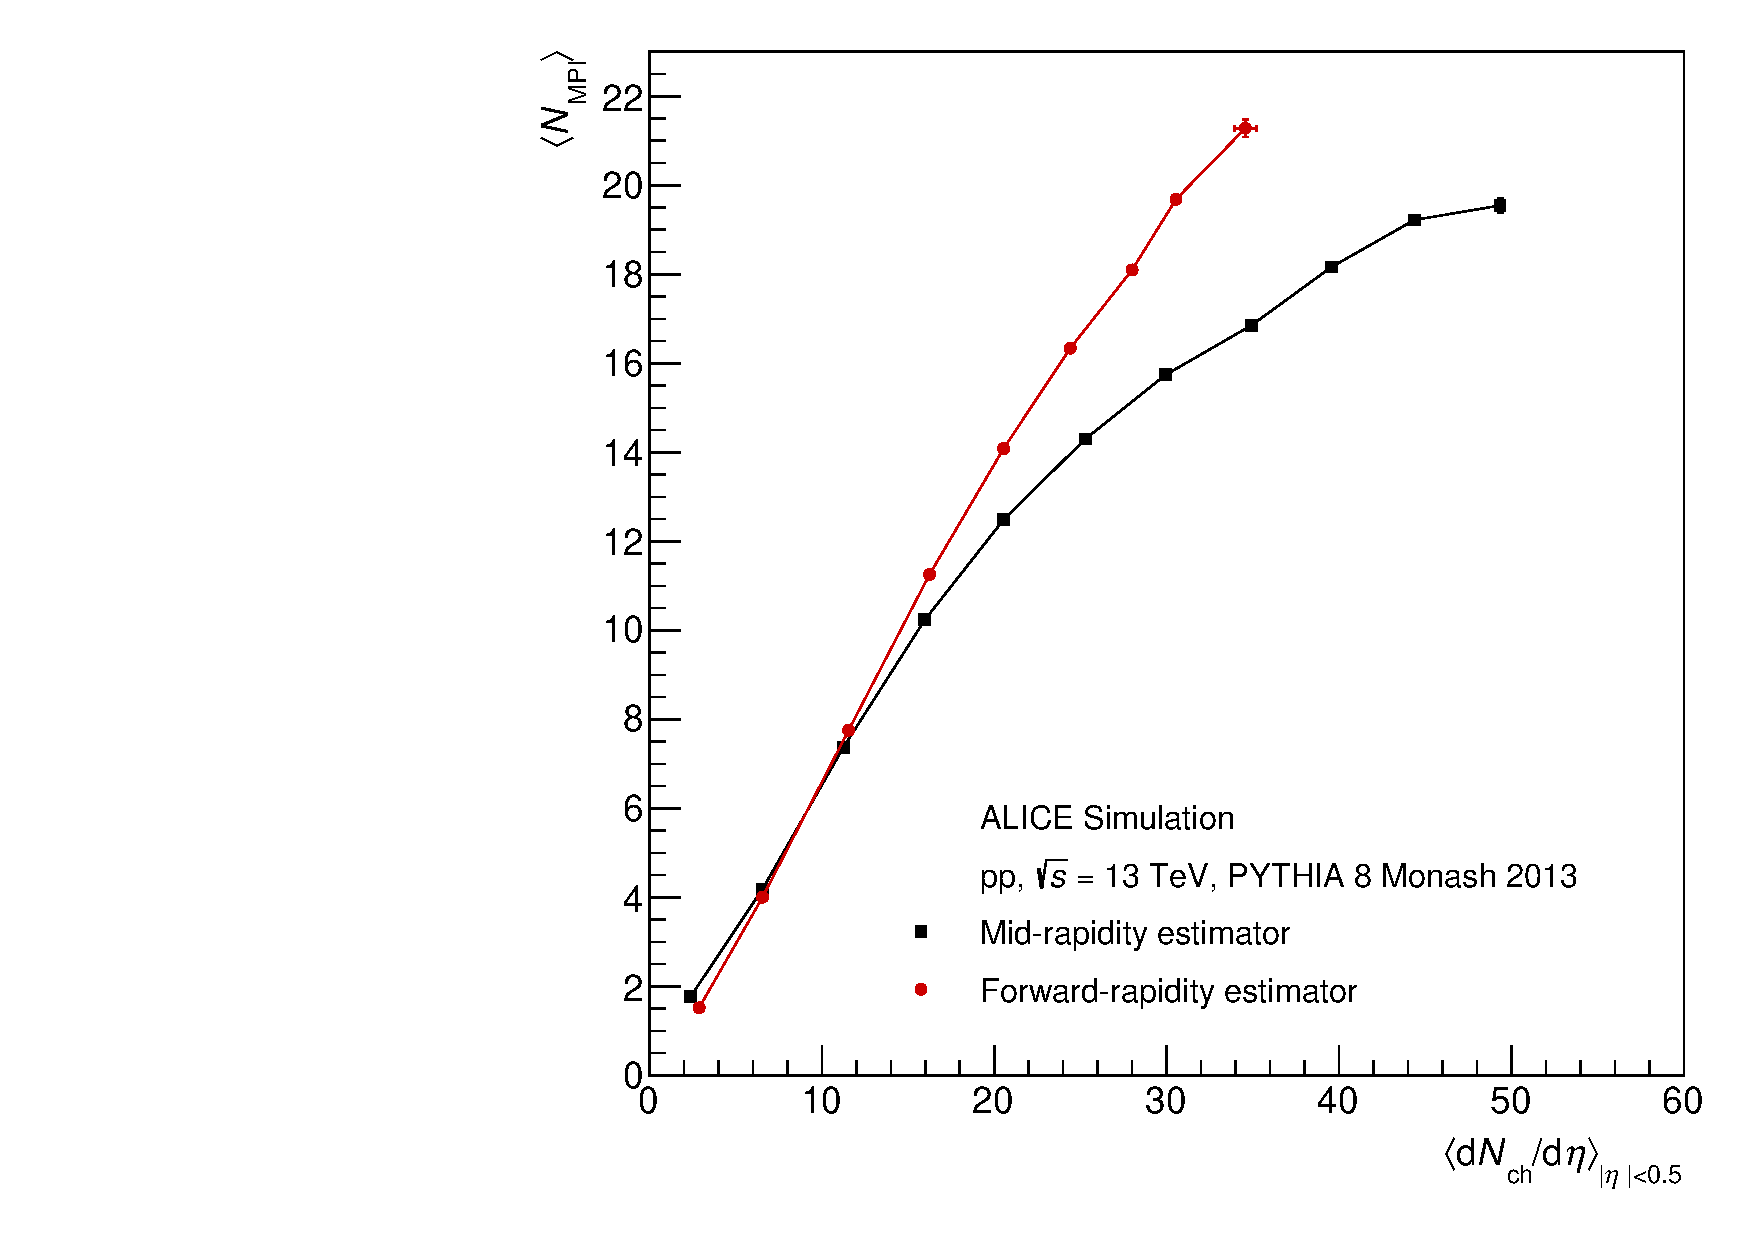
\includegraphics[width=.40\textwidth]{\imgpath/nmpi.pdf}}}
\caption{Mean number of MPIs as a function of multiplicity determined at mid-rapidity (black) and forward rapidity (red) in pp collisions at \sppt{13}, as simulated by Pythia 8. \cite{alicecollaborationALICEExperimentJourney2022}}
\label{fig:tracks:nmpi}
\end{figure}

\section{Used tracks}

The following tracks are often used in ALICE analyses and in the measurements within this dissertation:
\begin{itemize}
\item \spverb|ITSTPC2011|: The highest-quality ITS-TPC tracks, also referred to as ``global" tracks. They require TPC and ITS re-fit, TPC goodness-of-fit $\chi^2/n_\mathrm{cluster}^\mathrm{TPC} < 4$, ITS goodness-of-fit $\chi^2/n_\mathrm{cluster}^\mathrm{ITS} < 36$, $70$ crossed TPC rows, minimum $80\%$ of findable clusters based on geometrical considerations, clusters in the SPD, longitudinal DCA to the PV within $2$~cm, and no associated kink topology\footnote{In ALICE, decays of charged particles into one charged and one neutral daughter, e.g.\ $\pi^- \to \mu^- \bar{\nu_\mu}$, can be identified in the TPC from a characteristic ``kink" topology.}.
\item \spverb|TPCOnly|: Tracks with better azimuthal uniformity, which require TPC goodness-of-fit $\chi^2/n_\mathrm{cluster}^\mathrm{TPC} < 4$, $50$ crossed TPC rows, longitudinal DCA to the PV within $3.2$~cm, transverse DCA to the PV within $2.4$~cm, and no associated kink topology.
\item \spverb|V0daughter|: Secondary tracks used to find candidates for weakly-decaying \KOs and \LA (discussed further in Chapter~\ref{chap:analysis}), representing their charged daughters. They require a TPC re-fit, $70$ crossed TPC rows, and no kink topology.
\item Hybrid tracks: discussed below.
\end{itemize}

\subsection{Hybrid tracks}

For measurements requiring high track quality and momentum precision, such as for particle \pt spectra, the ITS-TPC tracks are usually used. As mentioned, these suffer from azimuthal non-uniformity due to the SPD acceptance. In situations where this is unacceptable, such as when using event shape observables or azimuthal topology classifications, ``hybrid tracks" can be used instead. These correspond to a union of ITS-TPC tracks and \textit{complementary tracks}, which are subjected to identical requirements save for the SPD cluster information. Furthermore, they must be constrained to the PV. A track can be classified as complementary only if it does not pass the ITS-TPC cuts first.

This union significantly improves the azimuthal uniformity, as displayed in Fig.~\ref{fig:tracks:hybrid}.

\begin{figure}%
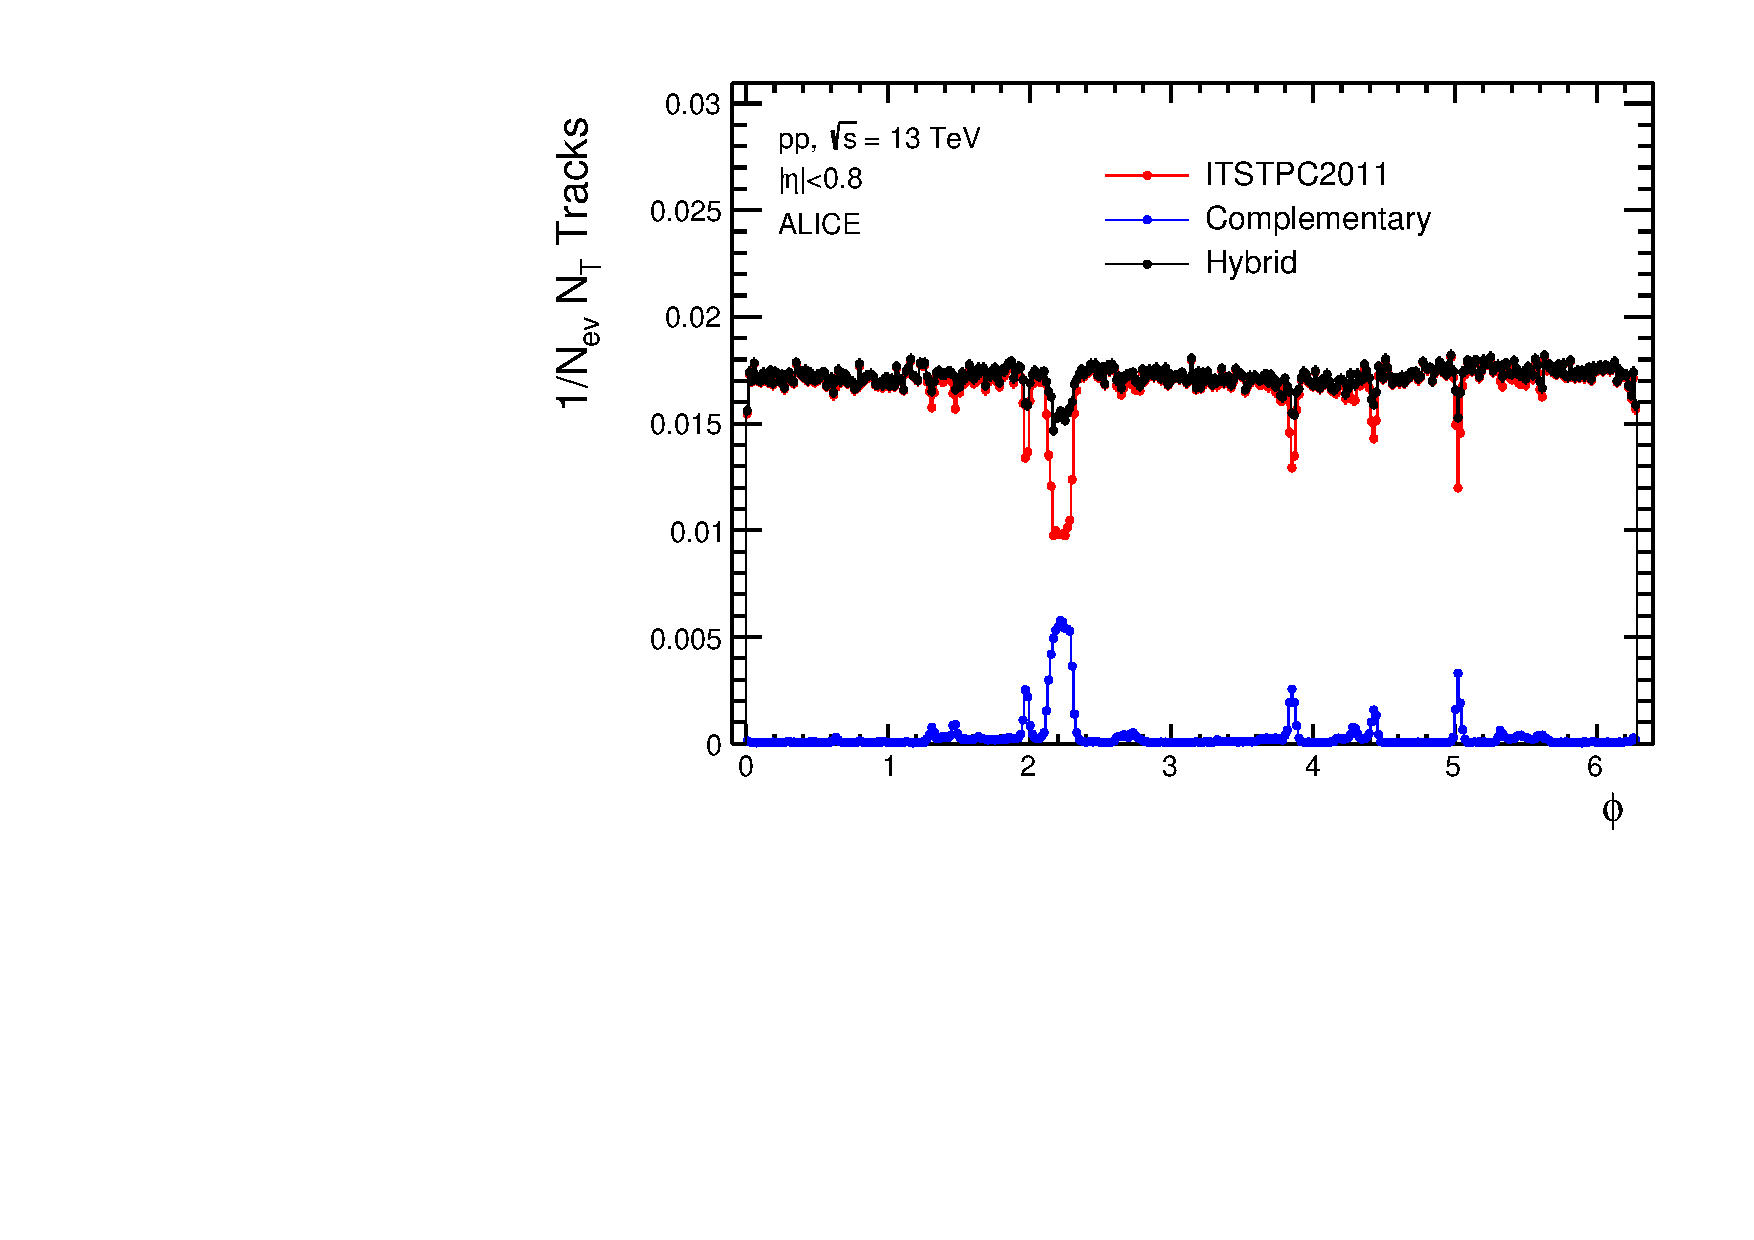
\includegraphics[width=.790\textwidth]{\imgpath/InfoRT_tracks.pdf}\\
\caption{Azimuthal distributions of the standard ITS-TPC tracks (red), complementary tracks (blue), and their union: hybrid tracks (black), in events used for measurements presented in this thesis. }
\label{fig:tracks:hybrid}
\end{figure}

\subsection{Geometrical cuts on tracks}

In measurements using a high-momentum trigger particle, additional geometrical constraints can be utilised to ensure the low-curvature particle trajectory does not significantly cover an inactive sector of the TPC.

In order to have just one set of requirements independent of the magnetic polarity and the particle charge, the azimuthal $\phi' = \phi$ is modified:
\begin{enumerate}
\item if $B<0$, then $\phi' = 2\pi - \phi'$,
\item then if $q<0$, then $\phi' = 2\pi - \phi'$,
\item and finally, $\phi' = \phi' + \frac{\pi}{18}$.
\end{enumerate}

Subsequently, the following cut is applied to reject tracks:
\begin{enumerate}
\item if $(\phi' \bmod \frac{\pi}{9}) < 0.12 / \pt + \frac{\pi}{18} + 0.035$,
\item AND if $(\phi' \bmod \frac{\pi}{9}) > 0.1 / \pt^2 + \frac{\pi}{18} - 0.025$ .
\end{enumerate}


\begin{tikzpicture}[node distance=1.25cm,>=Latex,rounded corners=5pt,thick, text width = 1.5cm]
\node[draw, rectangle] (clusterisation) {\small Clusterisation};
\node[draw, rectangle, right=of clusterisation] (first_pv) {\small First PV  (SPD)};
\node[draw, rectangle, right=of first_pv] (tpc_track) {\small TPC track  finding};
\node[draw, rectangle, right=of tpc_track] (tpc_its) {\small TPC track  matching in ITS};
\node[draw, rectangle, below=of clusterisation] (standalone_its) {\small Standalone ITS  track finding};
\node[draw, rectangle, right=of standalone_its] (track_propagation) {\small Track outwards  propagation};
\node[draw, rectangle, right=of track_propagation] (inwards_propagation) {\small Inwards propagation, final refit};
\node[draw, rectangle, below=of standalone_its] (final_pv) {\small Final PV finding};
\node[draw, rectangle, right=of final_pv] (secondary_vertices) {\small Secondary vertices (\VOs)};
\node[draw, rectangle, right=of secondary_vertices] (cascades) {\small Cascades};

 
        \draw[->] (clusterisation) -- (first_pv);
        \draw[->] (first_pv) -- (tpc_track);
        \draw[->] (tpc_track) -- (tpc_its);
        \draw[->] (tpc_its) -- (standalone_its);
        \draw[->] (standalone_its) -- (track_propagation);
        \draw[->] (track_propagation) -- (inwards_propagation);
        \draw[->] (inwards_propagation) -- (final_pv);
        \draw[->] (final_pv) -- (secondary_vertices);
        \draw[->] (secondary_vertices) -- (cascades);
\end{tikzpicture}